\section{Question Q1: what the entry \texorpdfstring{$(A^k)_{ij}$}{(A^k)_ij} represents}\label{sec:walkcount}

Q1 asks what the entry in row $i$ and column $j$ of a power of $A$ stands for.
We read the mark on the board as an exponent $k$ (\cref{conv:power}).

\subsection{The theorem}

\plain
Start in one town and make a fixed number of drives. Each drive follows one
road. You may turn round and go back along the road you just used. Multiply the road table by itself that many times. Look at the row of the first
town and the column of the second town. The number there counts the trips. It
counts trips, not tidy routes. A trip may pass the same town twice.

\begin{theorem}[walk counting]\label{thm:walkcount}
Let $G$ be a finite simple undirected graph with vertices $n_1,\dots,n_N$ and
adjacency matrix $A$. For every integer $k\ge1$ and all $i,j\in\{1,\dots,N\}$,
the entry $(A^k)_{ij}$ equals the number of walks of length $k$ from $n_i$ to
$n_j$.
\end{theorem}

The textbook has no such theorem (\cref{sec:intro}), so the proof below is our
own. The statement is also found in the University of Galway notes
(Theorem~1.1.3, \cite[p.~4]{galwaynotes}), in Bai's notes
(Theorem~1, \cite[p.~1]{bai2025adjacency}) and in Gotti's notes
(Proposition~2, \cite[p.~1]{gotti18211lecture27}). The method, induction on $k$
with the walks split by their last-but-one vertex, is the one those notes use
\cite{galwaynotes,gotti18211lecture27}.

\begin{proof}
We use induction on $k$. Let $W_k(i,j)$ denote the set of walks of length $k$
from $n_i$ to $n_j$, each written as a vertex sequence $(u_0,\dots,u_k)$ with
$u_0=n_i$, $u_k=n_j$ and every two consecutive vertices adjacent (see the remark
after \cref{def:walk}). The claim is $(A^k)_{ij}=|W_k(i,j)|$.

\emph{Base case, $k=1$.} A walk of length $1$ from $n_i$ to $n_j$ is a sequence
$(n_i,n_j)$ with $n_i$ and $n_j$ adjacent. There is exactly one such walk if
$e_{ij}\in E$ and none otherwise. So $|W_1(i,j)|=A_{ij}=(A^1)_{ij}$.

\emph{Induction hypothesis.} Let $k\ge1$ and suppose $(A^k)_{ir}=|W_k(i,r)|$ for
all $i$ and $r$.

\emph{Induction step.} By the definition of the matrix product,
$(A^{k+1})_{ij}=\sum_{r=1}^{N}(A^k)_{ir}A_{rj}$; each term will count the walks that
end with the drive from $n_r$ to $n_j$. Now take a walk $(u_0,\dots,u_k,u_{k+1})$ in $W_{k+1}(i,j)$
and let $n_r=u_k$ be its last-but-one vertex; $n_r$ is one of $n_1,\dots,n_N$.
Then $(u_0,\dots,u_k)$ lies in $W_k(i,r)$, and $n_r$ is adjacent to $n_j$.
Conversely, any walk in $W_k(i,r)$ followed by $n_j$, where $n_r$ and $n_j$ are
adjacent, is a walk in $W_{k+1}(i,j)$. So for each fixed $r$ the walks in
$W_{k+1}(i,j)$ with last-but-one vertex $n_r$ match one to one the pairs
consisting of a walk in $W_k(i,r)$ and the edge $e_{rj}$, where the edge exists
exactly when $A_{rj}=1$. Hence the number of such walks is $|W_k(i,r)|\,A_{rj}$,
which is $0$ when $A_{rj}=0$. Every walk has exactly one last-but-one vertex, so
the sets for different $r$ are disjoint and together cover $W_{k+1}(i,j)$.
Therefore
\[
|W_{k+1}(i,j)|=\sum_{r=1}^{N}|W_k(i,r)|\,A_{rj}
=\sum_{r=1}^{N}(A^k)_{ir}A_{rj}=(A^{k+1})_{ij}.
\]
The second equality is the induction hypothesis and the third is the definition
of the matrix product. This completes the induction.
\end{proof}

\emph{Why the proof is valid.} It uses three facts.
\begin{itemize}[leftmargin=1.5em]
  \item A walk of length $k+1$ is a walk of length $k$ plus one more edge.
  \item That edge exists exactly when the matrix entry is $1$.
  \item The matrix product sums over the possible last-but-one vertex.
\end{itemize}
Simplicity is used only to write a walk as its vertex sequence. Nothing forbids a
repeated vertex or a repeated edge, so the count is a count of walks. The
product $(A^k)_{ir}A_{rj}$ multiplies a count by $0$ or $1$ and never checks
which vertices the first part visited; this is why the proof cannot count paths.

\begin{remark}[length zero]\label{rem:zero}
With $A^0=I$, the entry $(A^0)_{ij}$ is $1$ if $i=j$ and $0$ otherwise. This
matches the walks of length $0$, which are the single vertices
(\cref{conv:zero}). The theorem is proved for $k\ge1$, and the case $k=0$ is that
convention.
\end{remark}

\plain
Every count of trips is a whole number, never below zero. A trip can be driven
backwards, so the count from the first town to the second equals the count from
the second to the first. A trip of two drives that starts and ends in the same
town goes out to a neighbour and straight back, so the count is the number of
roads at that town.

\begin{proposition}[more properties of $A^k$]\label{prop:powerprops}
Let $A$ be as in \cref{thm:walkcount}.
\begin{enumerate}[label=(\arabic*),leftmargin=2.2em]
  \item Every entry of $A^k$ is a nonnegative integer.
  \item $A^k$ is symmetric.
  \item $(A^2)_{ii}=d(n_i)$.
  \item The trace of $A^2$ (the sum of its diagonal entries) is $2|E|$.
\end{enumerate}
\end{proposition}

\begin{proof}
(1) $A$ has entries $0$ and $1$, and sums and products of nonnegative integers
are nonnegative integers. (2) The transpose $X^{T}$ of a matrix $X$ swaps its rows and columns; the transpose
of a product reverses the order of the factors, and $A^{T}=A$ by symmetry, so
$(A^k)^{T}=(A^{T})^k=A^k$. In walk terms, reversing a walk from
$n_i$ to $n_j$ gives a walk of the same length from $n_j$ to $n_i$, and this is
a one-to-one correspondence. (3) $(A^2)_{ii}=\sum_r A_{ir}A_{ri}=\sum_r A_{ir}^2=\sum_r A_{ir}$,
because the entries are $0$ or $1$, and this equals $d(n_i)$ by
\cref{prop:adjprops}(3). In walk terms, the walks of length $2$ from $n_i$ to
itself are $(n_i,n_r,n_i)$, one for each neighbour $n_r$. The Galway notes state
the same fact \cite[p.~4]{galwaynotes}. (4) The trace is the sum of the degrees,
which is $2|E|$ by \cref{thm:euler}.
\end{proof}

\subsection{A worked example: the board graph}\label{sec:board-example}

\plain
Take three towns in a row: the first has a road to the second, and the second
has a road to the third. We write the road table and multiply it by itself. Then
we list the trips behind a few of the numbers, to check that the table counts
them.

The board graph has the edges $n_1n_2$ and $n_2n_3$ (\cref{fig:board}). Its
powers, computed by script \cite{paperscript} and checked against an explicit
enumeration of all walks for $k=1,\dots,4$, are
\[
A=\matBoardA,\quad
A^2=\matBoardAtwo,
\]
\[
A^3=\matBoardAthree,\quad
A^4=\matBoardAfour .
\]
The matrix $A$ is symmetric with zero diagonal, and its row sums $1,2,1$ are the
degrees; their sum is $4=2|E|$.

\begin{figure}[ht]
\centering
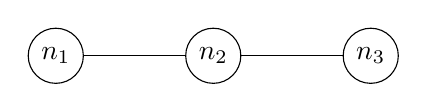
\begin{tikzpicture}[every node/.style={circle,draw,minimum size=7mm,inner sep=1pt}]
  \node (a1) at (0,0) {$n_1$};
  \node (a2) at (2,0) {$n_2$};
  \node (a3) at (4,0) {$n_3$};
  \draw (a1) -- (a2);
  \draw (a2) -- (a3);
\end{tikzpicture}
\caption{The board graph, the graph encoded by the board's matrix: two roads,
$n_1n_2$ and $n_2n_3$.}
\label{fig:board}
\end{figure}

\Cref{tab:boardwalks} lists the walks behind selected entries. Each count agrees
with the matrix.

\begin{table}[ht]
\centering
\caption{Walks behind selected entries of the powers of the board matrix. All
walks are written as vertex sequences. The last column lists those walks that
are paths in the course sense. Each value can be read off the printed matrices:
$(A^2)_{11}$ is the first entry of $A^2$, and so on.}
\label{tab:boardwalks}
\begin{tabular}{llp{5.6cm}p{3cm}}
\toprule
Entry & Value & Walks counted & Paths \\
\midrule
$(A^2)_{11}$ & 1 & $(n_1,n_2,n_1)$ & none \\
$(A^2)_{13}$ & 1 & $(n_1,n_2,n_3)$ & $(n_1,n_2,n_3)$ \\
$(A^2)_{22}$ & 2 & $(n_2,n_1,n_2)$, $(n_2,n_3,n_2)$ & none \\
$(A^2)_{12}$ & 0 & no walk & none \\
$(A^3)_{12}$ & 2 & $(n_1,n_2,n_1,n_2)$, $(n_1,n_2,n_3,n_2)$ & none \\
$(A^3)_{23}$ & 2 & $(n_2,n_1,n_2,n_3)$, $(n_2,n_3,n_2,n_3)$ & none \\
\bottomrule
\end{tabular}
\end{table}

\subsection{The board's drawing against the board's matrix}\label{sec:board-mismatch}

The board shows a drawing of three vertices beside its matrix
\cite{whiteboard1,whiteboard2}. \Cref{fig:boardredraw} redraws it. In plain terms, the board's drawing has three
roads and its matrix has two. We read the drawing as a line from $1$ to $2$
with an arrowhead at $2$, a line from $1$ to $3$, and a line between $3$ and
$2$; this reading has medium confidence. The matrix encodes only the edges
$n_1n_2$ and $n_2n_3$. \Cref{tab:mismatch} compares them pair by pair.

\begin{table}[ht]
\centering
\caption{Drawing against matrix, pair by pair.}
\label{tab:mismatch}
\small
\begin{tabular}{p{1.4cm}p{3.6cm}p{3.6cm}p{5.6cm}}
\toprule
Pair & Drawing & Matrix & Agree \\
\midrule
$n_1n_2$ & line, arrowhead at $n_2$ & $A_{12}=A_{21}=1$ & edge agrees; the arrowhead would make it directed, which a symmetric matrix does not \\
$n_2n_3$ & line & $A_{23}=A_{32}=1$ & agree \\
$n_1n_3$ & line & $A_{13}=A_{31}=0$ & disagree \\
\bottomrule
\end{tabular}
\end{table}

Following \cref{conv:matrix} the matrix is the example graph, and we do not hide
the mismatch. For comparison, the graph of the drawing without the arrowhead is
the triangle with edges $n_1n_2$, $n_1n_3$ and $n_2n_3$. Its powers
\cite{paperscript} are
\[
A_{\triangle}=\matTriA,\quad
A_{\triangle}^2=\matTriAtwo,
\]
\[
A_{\triangle}^3=\matTriAthree,\quad
A_{\triangle}^4=\matTriAfour .
\]
Both graphs are connected, but the counts differ. For example $(A^2)_{13}=1$ in
both graphs, while $(A^2)_{11}$ is $1$ for the board matrix and $2$ for the
triangle, which are the degrees of $n_1$ in the two graphs. In the triangle $(A^3)_{11}=2$
counts the closed walks $(n_1,n_2,n_3,n_1)$ and $(n_1,n_3,n_2,n_1)$, and
$(A^3)_{12}=3$ counts $(n_1,n_2,n_1,n_2)$, $(n_1,n_2,n_3,n_2)$ and
$(n_1,n_3,n_1,n_2)$, none of which is a path \cite{paperscript}. Which of the
two graphs the lecturer meant cannot be settled from the photos.

\subsection{Walks are not paths}\label{sec:notpaths}

\plain
The table counts every trip, including a trip that goes to a neighbouring town
and straight back. A tidy route visits each town at most once. So the table
gives more than the number of tidy routes. It can also give a positive number
when no tidy route exists.

Bai's notes say that the entry counts walks and not paths, because matrix
multiplication accumulates all edge sequences, including those that revisit
vertices \cite[p.~1]{bai2025adjacency}. The board graph gives three concrete
counterexamples to reading the entry as a number of paths; all three are in
\cref{tab:boardwalks} and the powers above \cite{paperscript}.

\begin{enumerate}[leftmargin=2.2em]
  \item $(A^2)_{11}=1>0$, but no path from $n_1$ to $n_1$ has length $2$: a
  sequence $(n_1,x,n_1)$ repeats $n_1$. The counted walk is $(n_1,n_2,n_1)$. In
  general $(A^2)_{ii}=d(n_i)>0$ whenever $n_i$ has a neighbour
  (\cref{prop:powerprops}(3)).
  \item $(A^3)_{12}=2$, but exactly one path joins $n_1$ to $n_2$, namely the
  edge, of length $1$, and no path has length $3$. The two counted walks are
  $(n_1,n_2,n_1,n_2)$ and $(n_1,n_2,n_3,n_2)$.
  \item $A^4$ is not the zero matrix although $N-1=2$ and a path has at most
  $N-1$ edges (\cref{prop:bound}). $A^4$ counts walks of length $4$, and a path with $4$ edges would need $5$
  different towns, but there are only $3$. So the entries of high powers cannot be
  counts of paths.
\end{enumerate}

\begin{remark}[where the count equals a path count]
For $k=1$ every walk is a path. For $k=2$ and $i\ne j$, the entry $(A^2)_{ij}$
is the number of paths of length $2$ from $n_i$ to $n_j$. The reason is that a
walk $(n_i,n_r,n_j)$ has distinct vertices exactly when $r\ne i$ and $r\ne j$,
and this holds automatically, because $n_r$ is adjacent to both and there are no
loops. For $k\ge3$ repeated vertices can occur even when $i\ne j$, as in the
second counterexample.
\end{remark}
